\chapter{训练感知机实现逻辑运算}

\section{感知机的逻辑运算}

简单的逻辑运算也是线性可分问题,感知机模型处理逻辑运算的超平面如下图所示
\begin{figure}[H]
    \centering
    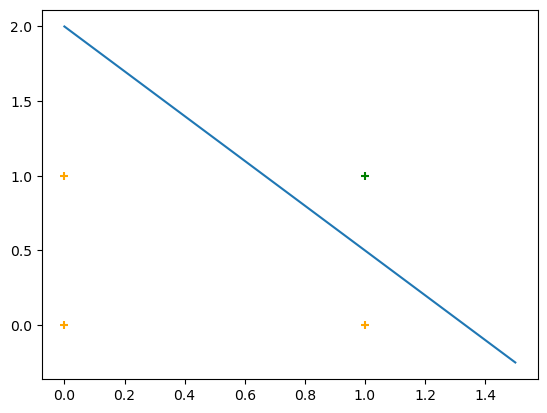
\includegraphics[scale=0.5]{figures/y_and.png}
    \caption{与运算}
\end{figure}

\begin{figure}[H]
    \centering
    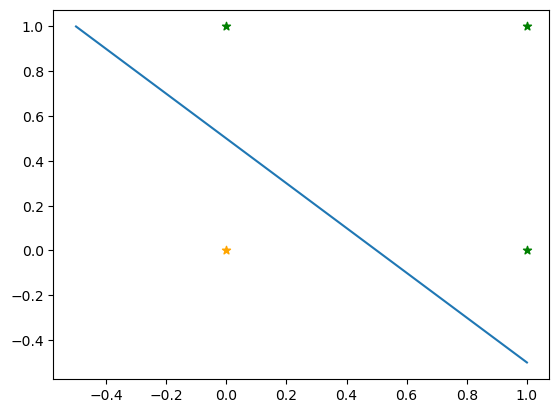
\includegraphics[scale=0.5]{figures/y_or.png}
    \caption{或运算}
\end{figure}



\section{异或问题}

单层感知机的一个问题是不能实现异或运算。

\begin{figure}[H]
    \centering
    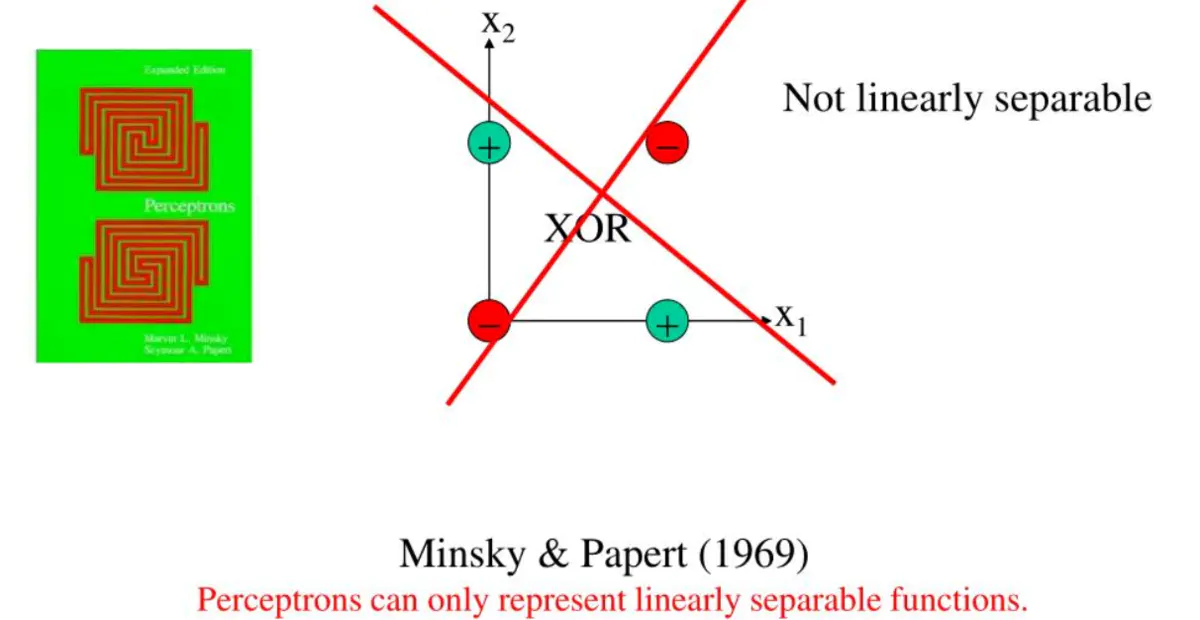
\includegraphics[scale=0.2]{figures/xor.png}
    \caption{异或问题}
\end{figure}

如下图所示,异或问题不是一个线性可分的问题,因此单层感知机在实现逻辑运算上存在缺陷。


\section{多层感知机}

多层感知器(英语:Multilayer Perceptron,缩写:MLP)是一种前向结构的人工神经网络,映射一组
输入向量到一组输出向量。MLP可以被看作是一个有向图,由多个的节点层所组成,每一层都全连接到下一层。
除了输入节点,每个节点都是一个带有非线性激活函数的神经元(或称处理单元)。一种被称为反向传播算法的
监督学习方法常被用来训练MLP。

多层感知器遵循人类神经系统原理,学习并进行数据预测。它首先学习
,然后使用权重存储数据,并使用算法来调整权重并减少训练过程中的偏差,即实际值和预测值之间的误差。主要优
势在于其快速解决复杂问题的能力。多层感知的基本结构由三层组成:第一输入层,中间隐藏层和最后输出层,输入元
素和权重的乘积被馈给具有神经元偏差的求和结点,主要优势在于其快速解决复杂问题的能力。
MLP是感知器的推广,克服了感知器不能对线性不可分数据进行识别的弱点。


\chapter{扩展阅读——通用近似定理}

在人工神经网络的数学理论中, 通用近似定理(或称万能近似定理)指出人工神经网络近似任意函数的能力。 
通常此定理所指的神经网络为前馈神经网络,并且被近似的目标函数通常为输入输出都在欧几里得空间的连续函数。
但亦有研究将此定理扩展至其他类型的神经网络,如卷积神经网络、放射状基底函数网络、或其他特殊神经网络。

此定理意味着神经网络可以用来近似任意的复杂函数,并且可以达到任意近似精准度。但它并没有说明要如何选择
神经网络参数(权重、神经元数量、神经层层数等等)来达到想近似的目标函数。

\subsection*{希尔伯特第十三问题}

德国数学家希尔伯特希望数学界能够证明:
\begin{equation}
    f^7+xf^3+yf^2+zf+1=0
\end{equation}

的七个解若表示成系数为$x,y,z$的函数,则此函数无法简化成两个变数的函数。

1957年,苏联数学家安德雷·柯尔莫哥洛夫(Андре́й Никола́евич Колмого́ров)的学生、当时19岁的弗拉基米尔·
阿诺尔德(Влади́мир И́горевич Арно́льд)解决了这个问题。柯尔莫哥洛夫证明每个有多个变元的函数可用有限个
三变元函数构作。阿诺尔德按这个结果研究,证明两个变元已足够。之后阿诺尔德和日本数学家志村五郎发表了一篇论文
(Superposition of algebraic functions (1976), in Mathematical Developments Arising From
 Hilbert's Problems)。这些结果后来被进一步发展,推导出人工神经网络中的通用近似定理,指人工神经网络能
 近似任意连续函数。

\subsection*{Kolmogorov–Arnold 表示定理}

在实分析和逼近理论中,Kolmogorov-Arnold 表示定理(Kolmogorov–Arn
old representation theorem,或叠加定理(superposition theorem))指
出,每个多元连续函数都可以表示为有限数量的单变量连续函数的两层嵌套叠加,这两个
层的函数分别称为内部函数和外部函数。它解决了希尔伯特第十三问题的一个更受约束但更一般的形式。
\footnote{米田引理、近似理论和迦瓦罗理论}

\chapter{参考阅读}

\begin{enumerate}
    \item 《 希尔伯特第 13 问题,Kolmogorov–Arnold representation theorem 和通用近似定理 》(Universal approximation theorem)\url{https://blog.csdn.net/qq_32515081/article/details/129569496} 
    \item 《 Understanding the Universal Approximation Theorem 》\url{https://towardsai.net/p/deep-learning/understanding-the-universal-approximation-theorem}
    \item 泛函分析:Stone–Weierstrass theorem 
    \item \url{https://www.jiqizhixin.com/articles/2021-09-07-6}
\end{enumerate}
